\begin{frame}
  \PN Para cada $j \geq 1$, sea $D_{j}$ la máquina siguiente:
  \begin{figure}[h]
    \centering
    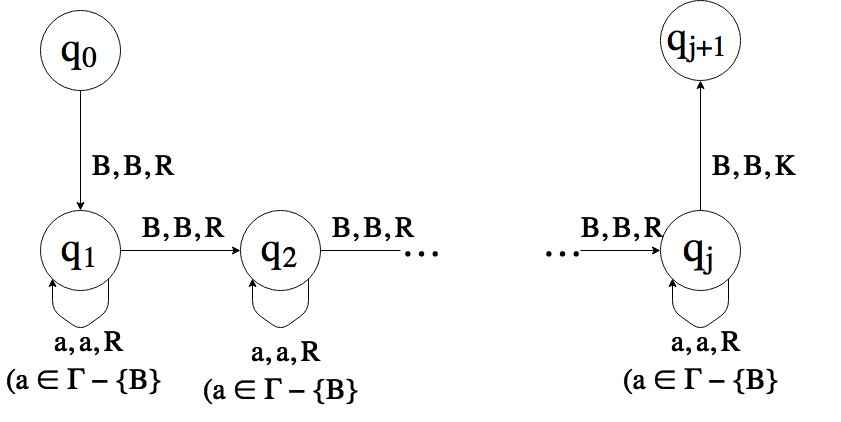
\includegraphics[scale=0.3]{graphics/figure_1.png}
  \end{figure}
  \PN Nótese que:
  \begin{equation*}
    \begin{array}{lcr}
      \alpha B \beta_{1} B \beta_{2} B \dotsc B \beta_{j} B \gamma &\overset{\ast}{\vdash}& \alpha B \beta_{1} B
        \beta_{2} B \dotsc B \beta_{j} B \gamma \\
      \ \ \uparrow && \uparrow \ \ \\
      \ \ q_{0} && q_{f}\ \
    \end{array}
  \end{equation*}
  \PN siempre que $\alpha, \gamma \in \Gamma^{\ast}, \beta_{1}, \dotsc, \beta_{j} \in (\Gamma - \{B\})^{\ast}$.
\end{frame}
